\documentclass[a4paper,12pt,leqno]{article}
\usepackage[utf8]{inputenc}
\usepackage[ngerman]{babel}

\usepackage{amsmath}
\usepackage{amsthm}
\usepackage{amsfonts}
\usepackage{amssymb}
\usepackage[left=3cm,right=2cm,top=2cm,bottom=1.5cm]{geometry}
\usepackage{parskip}
\usepackage{graphicx}
\usepackage{caption}
\usepackage{hyperref}
\usepackage{upgreek}
\usepackage{mathtools}
\usepackage{tikz}
\hypersetup{
    colorlinks,
    citecolor=black,
    filecolor=black,
    linkcolor=red,
    urlcolor=red
}

%%Code style
\usepackage{listings}
\usepackage{xcolor}
\definecolor{codegreen}{rgb}{0,0.6,0}
\definecolor{codegray}{rgb}{0.5,0.5,0.5}
\definecolor{codepurple}{rgb}{0.58,0,0.82}
\definecolor{backcolour}{rgb}{0.9,0.9,0.9}

\lstset{escapeinside={@}{@}}
\lstdefinestyle{mystyle}{
    backgroundcolor=\color{backcolour},   
    commentstyle=\color{codegreen},
    keywordstyle=\color{magenta},
    numberstyle=\tiny\color{codegray},
    stringstyle=\color{codepurple},
    basicstyle=\ttfamily\footnotesize,
    breakatwhitespace=false,         
    breaklines=true,                 
    captionpos=b,                    
    keepspaces=true,                 
    numbers=left,                    
    numbersep=5pt,                  
    showspaces=false,                
    showstringspaces=false,
    showtabs=false,                  
    tabsize=5
}

\lstset{style=mystyle}

\newcommand{\blue}[1]{\textcolor{blue}{#1}}
\newcommand{\orange}[1]{\textcolor{orange}{#1}}
\newcommand{\violet}[1]{\textcolor{violet}{#1}}
%%End code style

\title{Rechnerorganisation\\Zusammenfassung SS21}
\author{Felix Marx}

\begin{document}
\maketitle

{
%%Lokales Einfärben des Inhaltverzeichisses
\hypersetup{linkcolor=black}
\tableofcontents
}
\newpage

\section{Vorlesung 1}
\subsection{Begriffe}

\begin{figure}[h!]
\centering
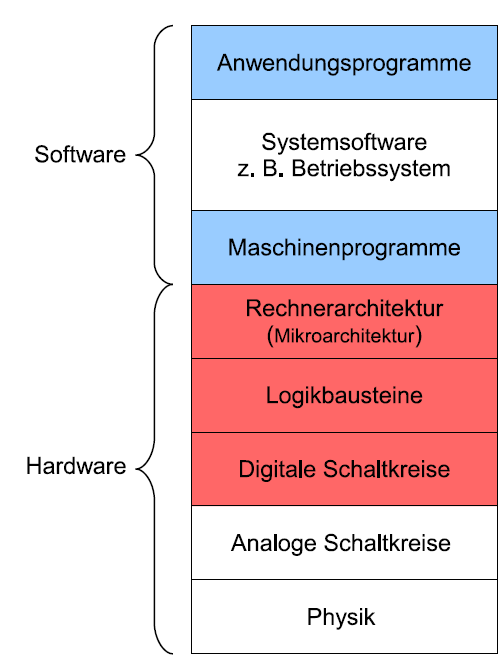
\includegraphics[scale=0.4]{Grafiken/Schichtenmodell.png}
\caption{Das Schichtenmodell ist eine abstrakte Darstellung eines Computers}
\end{figure}

\begin{itemize}
\item Abstraktion versteckt unnötige Details
\item Schichtenmodell teilt Dienstleistungen Schichten zu
	\begin{itemize}
	\item Schichten verrichten Arbeit für die nächst höhere
	\item Vorteile:
		\begin{itemize}
		\item Austauschbarkeit von Schichten
		\item Erfordert i.d.R. nur Kenntnis der aktuellen Schicht
		\item z.B. Gerätetreiber erfordern Wissen niedrigerer Schichten
		\end{itemize}
	\item Nachteile:
		\begin{itemize}
		\item ggf. geringere Leistungsfähigkeit
		\end{itemize}
	\end{itemize}
\end{itemize}
Computer ist ein Synonym für Datenverarbeitungssystem bzw. Rechnersystem:
\begin{quote}
"\emph{Ein Datenverarbeitungssystem ist eine Funktionseinheit zur
Verarbeitung und Aufbewahrung von Daten. Verarbeitung umfasst die
Durchführung \textbf{mathematischer}, \textbf{umformender}, \textbf{übertragender} und
\textbf{speichernder} Operationen.}"
\end{quote} 
Ein Rechnersystem unterscheidet sich von Messgeräten, dadurch dass es über ein ladbares Programm schrittweise eine Funktion ausführt.\\

Minimale Komponenten eines Rechnersystems:
\begin{itemize}
\item Prozessor
\item Speicher
\item I/O
\end{itemize}

\subsection{Geschichte}
{\small
\begin{tabular}{|l|l|l|}
\hline
Bezeichnung & Technik und Anwendung & Zeit\\
\hline
Abakus, Zahlenstäbchen & mechanische Hilfsmittel zum Rechnen & bis ca. 18. Jahrhundert\\
\hline
mechanische Rechenmaschinen & Apparate zum Rechnen & 1623 bis ca. 1960\\
\hline
elektronische Rechenanlagen & Lösen numerischer Probleme &  seit 1944\\
\hline
Datenverarbeitungsanlage & Texte und Bilder bearbeiten & seit ca. 1955\\
\hline
Informationsverarbeitungssystem & Bilder und Sprache erkennen (KI) & seit 1968\\
\hline 
\end{tabular}
}

Zuse Rechner:
\begin{itemize}
\item Z1 (1937): mechanische Rechenmaschine, bestehend aus
	\begin{itemize}
	\item Ein-/Ausgabewerk
	\item Rechenwerk
	\item Speicherwerk
	\item Programmwerk, Programm auf gelochten Filmstreifen
	\end{itemize}
\item Z2 (1939): Austausch der mechanischen Schaltglieder durch Relais (ca. 200) 10 Hz
\item Z3 (1941): erster funktionsfähiger Digitalrechner weltweit
\end{itemize}

\subsection{Ethik}
\begin{itemize}
\item Dual Use Problem (Ziviler und militärischer Einsatz)
\item Digitale Souveränität bezeichnet die Fähigkeit zu selbstbestimmtem Handeln und Entscheiden im digitalen Raum
	\begin{itemize}
	\item Selbstbestimmtes Handeln und Entscheiden
	\item Digitale Medien souverän zu nutzen (Medienkompetenz)
	\item Fähigkeit Vertrauenswürdigkeit und Integrität der Datenübertragung, -speicherung, -verarbeitung durchgängig zu kontrollieren
	\item Selbstbestimmung über die Nutzungsbestimmungen für seine Daten
	\item eigene Fähigkeiten mit Schlüsseltechnologien eigens Dienste und Plattformen zu betreiben
	\end{itemize}
\end{itemize}

\section{Vorlesung 2}
\subsection{Speicher}


Speicher können danach klassifiziert werden, ob sie für den Programmierer \textbf{explizit} oder nur \textbf{implizit/transparent} zugreifbar sind.
\begin{itemize}
\item explizite Nutzung
	\begin{itemize}
	\item interner Prozessorspeicher
		\begin{itemize}
		\item schnell, zur temporären Speicherung von Maschinenbefehlen und Daten
		\item direkter Zugriff durch Maschinenbefehle
		\item Halbleiter ICs\footnote{IC - Integrated circuit}
		\end{itemize}
	\item Hauptspeicher
		\begin{itemize}
		\item relativ groß und schnell, für Programme und Daten während der Ausführung
		\item direkter Zugriff durch Maschinenbefehle
		\item Halbleiter ICs
		\end{itemize}
	\item Sekundärspeicher
		\begin{itemize}
		\item sehr groß und langsam, für permanente Speicherung von Programmen und Daten
		\item indirekter Zugriff über I/O-Programme zur Übertragung in den Hauptspeicher
		\item Halbleiter ICs, Magnetplatten, optische Laufwerke, Magnetbänder
		\end{itemize}
	\end{itemize}
\item transparente Nutzung
	\begin{itemize}
	\item bestimmte Register auf dem Prozessor
	\item Cache Speicher
	\end{itemize}
\end{itemize} 

\begin{figure}[h!]
\centering
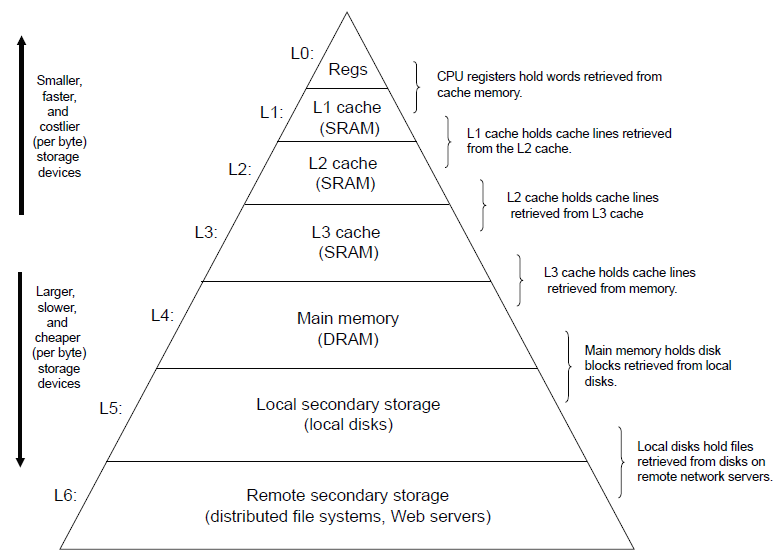
\includegraphics[scale=0.5]{Grafiken/Speicherhierarchie.png}
\caption{Speicherhierarchie, die Größe der Speicher nimmt nach oben ab, die Geschwindigkeit nimmt zu}
\end{figure}

\subsection{Einführung Assembler}

Maschinensprache (Assembler) ist ein primitives Paradigma\footnote{Paradigma bezeichnet ein übergeordnetes Prinzip, welches sich in Beispielen manifestiert}.\\
Das Programmiermodell von Assembler bezeichnet den Registersatz eines Prozessors, bzw. die Register, die durch Programme angesprochen werden können sowie die verfügbaren Befehle (Befehlssatz). Der Instruction Pointer (IP) und Program Counter (PC) zählen nicht zum Registersatz des Prozessors.\\

Komponenten des Rechnersystems:
\begin{itemize}
\item CPU/Prozessor: führt im Hauptspeicher abgelegte Befehle aus
\item ALU: Ausführung der Operationen
\item PC: Programmzähler, der auf den nächsten Maschinenbefehl im Hauptspeicher zeigt
\item Register: Schneller Speicher für Operanden
\item Hauptspeicher: Speichert Befehle und Daten
\item Bus Interface: Verbinden der einzelnen Komponenten
\end{itemize}

\subsubsection{Übersetzung und Ausführung}
\begin{figure}
\centering
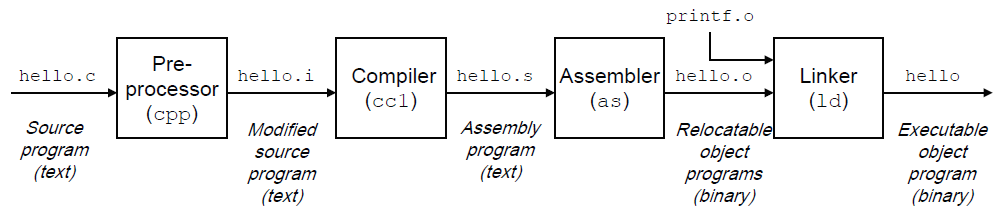
\includegraphics[scale=0.5]{Grafiken/Uebersetzungsprozess.png}
\caption{Die Phasen der Übersetzung eines C Programmes in binären Maschinencode}
\end{figure}

\begin{enumerate}
\item Preprocessor
	\begin{itemize}
	\item Aufbereitung durch Ausführung von Direktiven (mit \#) Inhalt der referenzierten Datei wird in Programmdatei kopiert
	\item Ausgabe: C-Programm mit der Endung .i
	\end{itemize}
\item Compiler
	\begin{itemize}
	\item Übersetzt das C-Programm name.i in ein Assemblerprogramm name.s
	\end{itemize}
\item Assembler
	\begin{itemize}
	\item Übersetzt name.s in Maschinensprache in das Objekt-Programm hello.o
	\end{itemize}
\item Linker
	\begin{itemize}
	\item Zusammenführen verschiedener Module (z.B. printf Funktion)
	\item Module werden zu einem ausführbaren Programm kombiniert
	\item Ausgabe des Bindeprogramms: name Datei, welche eine ausführbare Objekt-Datei, die in den Speicher geladen und ausgeführt werden kann
	\end{itemize}
\end{enumerate}

Nach dem Übersetzen kann die Objekt-Datei über die Shell ausgeführt werden. 
Dabei werden zunächst die Zeichen des Kommandos in die Register gelesen und den Inhalt dann in den Hauptspeicher gespeichert.\\
Anschließend werden Befehle und Daten schrittweise von der Festplatte in den Hauptspeicher kopiert.

\textbf{gcc programm.c} übersetzt das C-Programm\\
\textbf{gcc -S programm.c} generiert das Assemblerprogramm\\

Verschiedene Optimierungseinstellungen des Compilers lassen sich mit -O1 und -O2 dazuschalten.\\
Konstante Ausdrücke werden ggf. zur Compilezeit bereits ausgewertet und in Assembler durch das Ergebnis ersetzt.\\
Wir unterscheiden die Befehle eines Rechnersystems in \textbf{CISC} - Complex Instruction Set Computer und \textbf{RISC} - Reduced Instruction Set Computer.\\
CISC besitzen viele komplexe Befehle, wohingegen RISC weitgehend Befehle mit identischer Ausführungszeit hat um effizientes Pipelining zu ermöglichen. RISC werden auch als Load/Store-Architekturen bezeichnet.\\

\begin{figure}[h!]
\centering
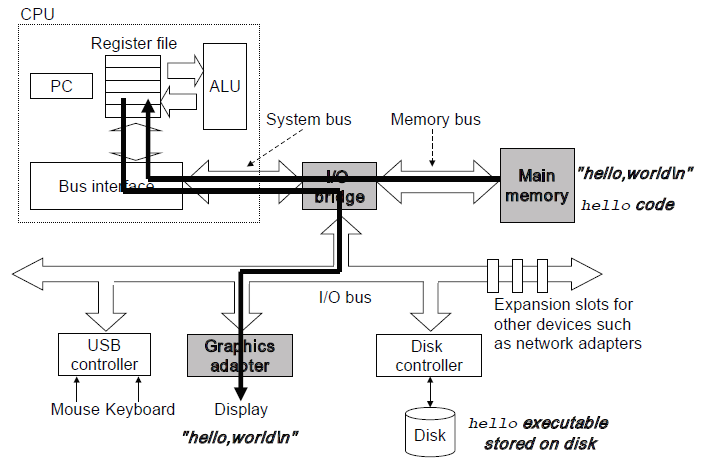
\includegraphics[scale=0.6]{Grafiken/Ausfuehrung-eines-Programmes.png}
\caption{Im letzen Schritt der Ausführung werden die Maschinenbefehle des Programmes ausgeführt}
\end{figure}

Weiterhin beeinflusst die Struktur eines Prozessors die Leistungsfähigkeit und Kosten des Rechnersystems massiv.\\
Wir Teilen Rechnersysteme nach der Anzahl der Operanden in einem Maschinenbefehl ein (n-Adressmaschinen).\\

CISC-Maschine: Intel Architektur\\
2-Adressmaschine: Intel Architektur\\
RISC-Maschine: ARM Architektur\\
3-Adressmaschine: ARM Architektur\\

ARM besitzt 16 Register und ein Current Processor Status Register (CPSR). Dabei sind:
\begin{itemize}
\item R0: das Rückgaberegister
\item R1 - R12: frei verwendbar
\item R13: der Stack Pointer (sp) zeigt auf den Kopf des Stacks
\item R14: das Link Register (lr) zeigt auf die Rücksprungadresse
\item R15: der Programm Counter (pc) speichert die aktuelle Programmadresse
\end{itemize}

Wir unterscheiden in der Speicherorganisation: Big-Endian und Little-Endian.\\
Bei \textbf{Big-Endian} werden die Bytes vom höchstwertigen Ende an gezählt.\\
Bei \textbf{Little-Endian} werden die Bytes vom niedrigstwertigen Ende an gezählt.\\
 
In der Adressnummerierung hat bei Big-Endian das MSB also die Adresse 0, bei Little-Endian hat das LSB die Adresse 0.\\
ARM ist byte-adressiert und verwendet i.d.R. Little-Endian (kann aber manuell festgelegt werden). Ein Wort ist dabei 32 Bit = 4 Bytes lang, somit sind Wortadressen immer Vielfache von 4.

\section{Vorlesung 3}
\subsection{Grundlegende Assembler Befehle}
Direktwerte, d.h. Werte welche direkt als solche im Assemblercode geschrieben werden, müssen im Zweierkomplement als 12 Bit Wert repräsentierbar sein.
\subsubsection{load}
Mit dem Ladebefehl ldr (load word) wird ein Datenwort von einer Speicheradresse gelesen und in das angegebene Register geschrieben. 
\begin{lstlisting}
ldr r1, [r2, #4]
\end{lstlisting}

Im obigen Beispiel wird ein Datenwort von der Adresse (r2 + 4) gelesen und in das Register r1 geschrieben. Also das zweite\footnote{Da die Datenworte 4 Byte lang sind} Datenwort im Register r2.\\
Gelesen als Basisadresse r2 plus Offset 4.\\
Als Basisadresse darf jedes Register verwendet werden.\\
Der Offset kann auch Hexadezimal angegeben werden (z.B. \#0xC für \#12).\\
Auch eine Angabe durch ein Register ist erlaubt.

\subsubsection{store}
Mit dem Speicherbefehl str (store word) wird ein Datenwort in das zweite Register plus Offset geschrieben.
\begin{lstlisting}
str r2, [r3, #0x14]
\end{lstlisting}

Im obigen Beispiel wird das an der Adresse von r2 gespeicherte Datenwort an die Adresse r3 plus 20 = 0x14 geschrieben.
Der Befehl hat auch eine Byte Variante strb, welche das LSB der gegebenen Adresse an das Ziel schreibt.

\subsubsection{mov}
Schreibt den angegebenen Wert in das Zielregister.
\begin{lstlisting}
mov r1, #0
\end{lstlisting}
Im obigen Beispiel wird der Wert 0 an die Adresse r1 geschrieben.

\subsubsection{add}
Addiert zwei Werte zusammen und schreibt das Ergebnis an die Ergebnisadresse.
\begin{lstlisting}
add r0, r0, #4
\end{lstlisting}
Im obigen Beispiel wird der Wert an der Adresse r0 um 4 erhöht und dann an die Adresse r0 geschrieben. 

\subsubsection{sub}
Subtrahiert zwei Werte von einander und schreibt das Ergebnis an die Ergebnisadresse.

\begin{lstlisting}
sub r3, r6, r9
\end{lstlisting}
Im Beispiel wird der Wert an der Adresse r9 vom Wert an der Adresse r6 subtrahiert und an die Adresse r3 geschrieben. 

\subsubsection{mul}

Multipliziert die beiden Operanden mit einander und speichert die least significant 32 Bit an die Ergebnisadresse.
\begin{lstlisting}
mul r1, r2, r3
\end{lstlisting}
Im Beispiel wird der Wert an der Adresse r2 mit dem Wert an der Adresse r3 multipliziert und an die Adresse r1 geschrieben.

\subsubsection{lsl}
Ein logischer Shift nach links\footnote{Beim logischen Shift wird der Überfluss abgeschnitten und die leeren Stellen mit 0'en aufgefüllt}. Entspricht einer Multiplikation um die Zahl $2^n$. Dabei wird der Wert im zweiten Register um den Wert im dritten Operanden nach links geshifted.
\begin{lstlisting}
lsl r1, r2, r3
lsl r1, r2, #1
\end{lstlisting}
Wenn der dritte Operand ein Register ist, wird nur das least significant byte beachtet. Ist der Operand ein Direktwert, so darf dieser maximal 32 sein.

\subsubsection{lsr}
Ein logischer Shift nach rechts. Entspricht einer Division um die Zahl $2^n$. Dabei wird der Wert im zweiten Register um den Wert im dritten Operanden nach rechts geshiftet.
\begin{lstlisting}
lsr r1, r2, r3
lsr r1, r2, #1
\end{lstlisting}
Die selben Einschränkungen wie bei lsl gelten.

\subsubsection{ORR/AND}
Ein logisches bitweises OR bzw. AND, das Ergebnis wird in das erste Register geschrieben. Der zweite Operand muss ein Register sein, der dritte Operand ist beliebig.
\begin{lstlisting}
AND r1, r2, #0x1234
ORR r1, r2, r3
\end{lstlisting}


\subsection{Flags}
Wichtige Flags sind:
\begin{itemize}
\item CF Übertragsflag (Carryflag)
\item ZF Nullflag (Zeroflag)
\item SF Vorzeichenflag (Signflag)
\item OF Überlaufflag (Overflowflag)
\end{itemize}

\textbf{Unterscheidung zwischen CF und OF Flags:}\\
Overflowflag (OF) wird gesetzt, wenn wir z.B. zwei positive Zahlen addiert werden, aber aufgrund eines Speicherüberflusses das Ergebnis negativ ist.\\

Carryflags (CF) werden gesetzt, wenn wir z.B. eine positive und eine negative Zahl addieren, und das Ergebnis noch korrekt darstellbar ist, aber in der binären Addition ein Bit überläuft. Zum Beispiel so:
\begin{tabbing}
---\=---\=0000----\=\kill
\>\>0101\>5\\
\>\>1111\>-1\\
\>\>------\\
\>1\>0100\>4
\end{tabbing}

Ist das Ergebnis negativ wird das Signflag (SF) auf 1 gesetzt.

\subsection{Assembler Sprungbefehle}

\subsubsection{Unbedingte Sprünge}
Unbedingte Sprünge (b) werden immer ausgeführt sobald sie im Programmablauf erreicht werden.\\
Die Sprungadressen werden mit Labels im Programmcode festgelegt und mit einem Doppelpunkt abgeschlossen.
\begin{lstlisting}
mov r1, #4
b label
sub r1, r1, #2
label:
...
\end{lstlisting}

\subsubsection{beq}
Der Sprung wird nur ausgeführt falls das Zeroflag (ZF) gesetzt ist.\\
Dabei wird i.d.R. vor dem Sprungbefehl der Vergleichsbefehl cmp aufgerufen, welcher zwei Werte durch Subtraktion vergleicht.
Der Befehl cmp muss als ersten Parameter immer ein Register bekommen, der zweite Parameter ist beliebig.
\begin{lstlisting}
mov r0, #4
cmp r0, #8 /* setzte Flags auf Basis von r0 - 8 = -4 @$\Rightarrow$@ NZCV = 1000 */
beq label /* Hier kein Sprung, da Z != 1 */
...
label:
\end{lstlisting}

\subsection{If-Verzweigungen}
In Hochsprache:
\begin{lstlisting}
if (r0 == r1)
	r2 = r3 + 1;
r2 = r2 - r3;
\end{lstlisting}

In Assembler negieren wir die Bedingung, sodass falls diese erfüllt ist wir den konditionalen Block überspringen können.
\begin{lstlisting}
cmp r0, r1
bne L1 /* Springt falls Werte ungleich @$\Leftrightarrow$@ Z = 0 */
add r2, r3, #1
L1:
sub r2, r2, r3
\end{lstlisting}

\subsection{If-Else-Verzweigungen}
In Hochsprache:
\begin{lstlisting}
if (r0 == r1)
	r2 = r3 + 1;
else
	r2 = r2 - r3;
\end{lstlisting}

In Assembler negieren wir wieder die Bedingung, um somit direkt in den else Case zu springen, hängen ans Ende des if-Blockes noch einen unbedingten Sprungbefehl, um den else-Block zu überspringen.
\begin{lstlisting}
cmp r0, r1
bne L1
add r2, r3, #1
b L2
L1:
sub r2, r2, r3
L2:
\end{lstlisting}

\subsection{while-Schleifen}
In Hochsprache:
\begin{lstlisting}
int pow = 1;
int x = 0;
while (pow != 128) {
	pow = pow * 2;
	x = x + 1; 
}
\end{lstlisting}
In Assembler überprüfen wir nach unserer Einstiegsmarke, ob die negierte Fortsetzungsbedingung erfüllt ist und beenden die Ausführung im positiven Fall. Sonst wird der Schleifenkörper ausgeführt und wir springen unbedingt zur Einstiegsmarke zurück.
\begin{lstlisting}
mov r0, #1
mov r1, #0
WHILE:
cmp r0, #128
beq DONE
lsl r0, r0, #1 /* pow = pow * 2 */
add r1, r1, #1 /* x = x + 1 */
b WHILE
DONE: 
\end{lstlisting}

\subsection{for Schleifen}
In Hochsprache:
\begin{lstlisting}
int sum = 0;
int i;
for (i = 0; i < 10; i = i + 1) {
	sum = sum + i;
}
\end{lstlisting}

In Assembler prüfen wir direkt nach der Einstiegsmarke, ob die negierte Fortsetzungsbedingung erfüllt ist und beenden im positiven Fall. Sonst wird der Schleifenkörper ausgeführt und im Anschluss Zähler entsprechend angepasst. Dann springen wir unbedingt zur Einstiegsmarke zurück.
\begin{lstlisting}
mov r1, #0
mov r0, #0
FOR:
cmp r0, #10
bge DONE /* Springe falls der gilt r0 > 10 @$\Leftrightarrow$@ N != 0 && Z = 0 */
add r1, r1, r0 /* sum = sum + i */
add r0,r0, #1 /* i = i +1 */
b FOR
DONE:
\end{lstlisting}

\section{Vorlesung 4}

\subsection{Nutzen des Hauptspeichers}
Anstatt Werte als Direktwerte zu benutzen, können sie auch als Variablen im Datenbereich des Programms definiert werden.
\begin{lstlisting}
.data /* Datenbereich */
var1: .word 5 /* Variable 1 im Speicher mit Wert 5 */
var2: .word 12 
var3: .word 15

.global main /* Definition Einsprungpunkt Hauptprogramm */

main: /* Hauptprogramm */
	ldr r0, var1 /* laedt Wert von var1 in r0 */
	
	ldr r1, adr_var2 /* laedt Adresse von var2 in r1 */
	ldr r2, [r1] /* Laedt den Inhalt von Adresse r1 in r2 */

	ldr r3, =var3 /* Laedt die Adresse von var3 direkt in r3 */
	ldr r4, [r3] /* Laedt den Inhalt von Adresse r3 in r4 */
	
	add r0, r0, r2
	bx lr /* Springe zurueck zum aufrufenden Programm */

adr_var2: .word var2 /* Adresse von Variable 2 */
\end{lstlisting}
Die Daten in var1 werden direkt adressiert, die Daten in var2 werden indirekt adressiert. Die Abkürzung für die Adresse einer im Datenbereich definierten Variable ist:\\ =variablenname, wie bei var3 dargestellt.\\

Die einzelnen Registerfelder liegen direkt übereinander, sodass wenn wir Zeile 15 durch:
\begin{lstlisting}
ldr r4, [r3, #8]
\end{lstlisting}
ersetzen, die Adresse (r3 + 8) = (r2 + 4) = r1 erhalten und von dieser Adresse den Wert 12 an r4 schreiben.

\subsection{Arrays}
Arrays oder auch Datenfelder können als konsekutive Datenwörter aufgefasst werden welche übereinander im Speicher liegen, sodass der Index eines einzelnen Feldes dem Offset von der Basisadresse entspricht.\\
Dabei lädt man i.d.R. die Basisadresse des Arrays in ein Register und den Index in ein weiteres. Um nun auf einzelne Datenwörter zuzugreifen, muss der Index um die Wortbreite (4 Bytes) multipliziert werden.
\begin{lstlisting}
mov r0, #0x11111 /* Basisadresse des Arrays */
mov r1, #0 /* Index i */
...
lsl r2, r1, #2 /* r2 = i * 4 (Offset) */
ldr r3, [r0, r2] /* Laedt das indizierte Arrayelement */
\end{lstlisting}

\subsection{Unterprogramme}

Unterprogramme helfen bei der strukturierten Programmierung, indem Teile des Hauptprogrammes in Teilprogramme (TP) ausgelagert werden.\\
Man unterscheidet zwischen Makrotechnik und Unterprogrammtechnik.
Bei der \textbf{Makrotechnik} wird das Programm an den benötigten Stellen einkopiert, dabei wird dem TP, dem sogenannten Makro, ein Name zugeordnet (Makroname). An den Stellen wo das Makro einkopiert werden soll, wird der Makroname genannt.\\
Bei der \textbf{Unterprogrammtechnik} ist das Unterprogramm (UP) nur einmal im Code vorhanden. Es wird durch eine Marke (Unterprogrammname) gekennzeichnet. Soll das UP aufgerufen werden, erfolgt ein Sprungbefehl mit der Marke als Operand.
Am Ende des UPs erfolgt die Rückkehr in das aufrufende Programm mittels speziellem Sprungbefehl (z.B. bx). Die Rückkehradresse wird in Registern oder auf dem Stack gespeichert.\\

Lokale Variablen werden i.d.R. über den Stack realisiert.
Als Regel für Prozeduraufrufe gilt:
\begin{itemize}
\item Der Aufrufer übergibt Argumente an den Aufgerufenen und springt zum Aufgerufenen
\item Der Aufgerufene führt eine Funktion/Prozedur aus und gibt das Ergebnis an den Aufrufer zurück (r0)
\item Die Rücksprungadresse liegt direkt hinter der Aufrufstelle
\item Der Aufgerufene darf keine Register oder Speicherstellen überschreiben, die im Aufrufer genutzt werden
\item Aufgerufene Unterprogramme dürfen keine unbeabsichtigten Seiteneffekte haben
\end{itemize}

\begin{lstlisting}
main:
mov r0, #4 /* Argument 0 ist 4 */
mov r1, #30 /* Argument 1 ist 30 */
bl sum /* Funktionsaufruf, bl legt Rueckkehradresse in r14 (lr) */
mov r2, r0 /* r0 ist der Rueckgabewert */

sum: /* Unterprogrammname */
add r2, r0, r1 /* Fuehrt seine Funktion aus */
mov r0, r2 /* Legt Rueckgabewert in r0 ab */
mov pc, lr /* Ruecksprung zum Aufrufer */
\end{lstlisting}

\section{Vorlesung 5}
\subsection{Stack}
Der Stack wächst bei ARM nach unten, d.h. von hohen zu niedrigen Speicheradressen.
Der Stackpointer: r13 (sp) zeigt auf das oberste Element des Stacks.\\

\begin{lstlisting}
sub sp, sp, #8 /* reserviert Speicher fuer 2 Woerter auf dem Stack */
str r8, [sp, #4] /* sichert den Wert von r8 auf dem Stack */
str r7, [sp] 
...
ldr r7, [sp] /* stellt den Wert von r7 wieder her */
ldr r8, [sp, #8] /* stellt den Wert von r8 wieder her */
add sp, sp, #8 /* gibt den Speicher auf dem Stack wieder frei */
\end{lstlisting}

Werden weiter Unterprogramme aufgerufen, muss auch die Rücksprungadresse lr auf dem Stack gesichert werden, sonst geht diese beim Prozeduraufruf verloren.\\


\begin{figure}
\centering
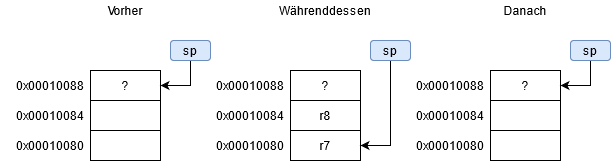
\includegraphics[scale=0.7]{Grafiken/stackManipulation.png}
\caption{Repräsentation des Stacks vor, während und nach der Programmausführung}
\end{figure}

Kurzschreibweisen (Pseudoinstruktionen) für das reservieren/freigeben von Speicher und dem ablegen/wiederherstellen von Wörtern sind die Instruktionen:
\begin{lstlisting}
push {lr} /* Ablegen der Ruecksprungadresse*/
...
pop {lr} /* Wiederherstellen der Ruecksprungadresse */
\end{lstlisting}

\subsection{Rekursion}
Bei einer rekursiven Programmausführung repräsentiert die Anzahl an Rücksprungadressen auf dem Stack im wie vielen Aufruf wir uns befinden. Der Ablauf eines Unterprogramms wird auch als Inkarnation (wiederholter Unterprogrammaufruf) bezeichnet.\\
Auszug einer rekursiven Funktion:
\begin{lstlisting}
.text /* markiert den Beginn eines Code Segments */
fak:      push {r0, lr}
		cmp r0, #1 /* Rekursionsende pruefen */
		blt else /* branch less @$\Leftrightarrow$@ N = 1 */
		sub r0, r0, #1 /* n-1 */
		bl fak /* rekursiver Funktionsaufruf */
		/* Ruecksprungadresse beim zurueckgehen */

RA_2:	ldr r1, [sp, #4] /* laden von n */
		mul r0, r1, r0 /* fak(n-1) * n */
fin:      pop {lr} /* laden der Rueckkehradresse */
		add sp, sp, #4 /* Freigeben des Stackspeichers */
		bx lr	/* Sprung zum Aufrufer */
		
else:	mov r, #1	/* Rekursionsanker */
		b fin /* Rekursionsende, abbauen des Stacks */
\end{lstlisting}

\section{Vorlesung 6}
\subsection{OpenMP}
OpenMP ist eine Sammlung von Compiler-Anweisungen (Direktiven) und Bibliotheksfunktionen für die Thread Programmierung.\\
Es ist eine Kombination von C, C++ und Fortran. Dadurch wird threadparalleles Arbeiten ermöglicht.\\
OpenMP startet als einzelner Thread und forkt für einzelne parallele Programmabschnitte zusätzliche Threads. Nach Abschluss joinen die Threads wieder zusammen. Dies wird auch \textbf{Fork-Join-Programmiermodell} bezeichnet.\\

\begin{lstlisting}
#include<omp.h> /* OpenMP Library */
...
#pragma omp parallel for private(x) reduction(+:sum)
for( i = 0; i < num_steps; i++) {
	x = (i + 0.5) * step;
	sum += 4.0 / (1.0 + x * x)
}
...
\end{lstlisting}

\subsection{Assembler}
Der Assembler ist ein Programm, dass die Aufgabe hat, Assemblerbefehle in Maschinencode zu transformieren und dabei symbolische Namen Maschinenadressen zuweist und eine oder mehrere Objektdatei(en) erzeugt.\\
Varianten sind Crossassembler, welche Maschinencode für eine andere Plattform erzeugen als sie gerade laufen, sowie Disassembler welche Maschinensprache in Assemblersprache übersetzen.\\

Die Übersetzung erfolgt in zwei Schritten:\\
1. Schritt:
\begin{itemize}
\item Auffinden von Marken um Beziehungen zwischen symbolischen Namen und Adressen zu kennen (Syntax- und Kontextanalyse)
\item Übersetzen jedes Assemblerbefehls durch Kombination der Opcodes\footnote{Nummer des entsprechenden Maschinenbefehls}, Bezeichner und Marken zu legalen Instruktionen (Codegen)
\end{itemize}
2. Schritt: Erzeugen einer oder mehrerer Objektdateien. Diese ist meist nicht ausführbar, da sie auf Funktionalitäten anderer Dateien angewiesen ist.

Probleme bei den Schritten:
\begin{itemize}
\item Bei Schritt 1 sind zukünftige Marken nicht bekannt $\rightarrow$ Aufteilen in Syntax- und Kontextanalyse (2 Läufe)
\item Bei Schritt 2 werden in der Objektdatei absolute Adressen verwendet
	\begin{itemize}
	\item Programm kann direkt ausgeführt werden, aber der Speicherort muss vorher bekannt sein
	\item Nachträgliches verschieben des Programms ist nicht möglich
	\end{itemize}
\item Bei Schritt 2 werden relative Adressen verwendet, und die aktuelle Adresse bei Programmbeginn übergeben
	\begin{itemize}
	\item Erzeugt ggf. mehrere Objektdateien
	\item Adressen werden relativ zu den einzelnen Objektdateien vergeben
	\item Vor Ausführung sind weitere Transformationsschritte nötig, Aufgabe des Binders/Linkers und Laders
	\end{itemize}
\end{itemize}

\subsection{Objekt-Programme}
Wir unterscheiden:
\begin{itemize}
\item Relocatable object files: Enthält binären Code und Daten, sodass diese mit anderen relocatable object files zu einem ausführbaren Objektfile zusammengefügt werden können
\item Executable object files: Enthält binären Code und Daten, welche direkt in den Speicher kopiert und ausgeführt werden können
\item Shared object files: Spezialfall der relocatable object files, welche in den Speicher geladen werden können und dynamisch mit anderen Objekt-Files zusammengeführt werden können 
\end{itemize}
In der Regel generieren Compiler und Assembler relocatable object files.

\begin{figure}[h!]
\centering
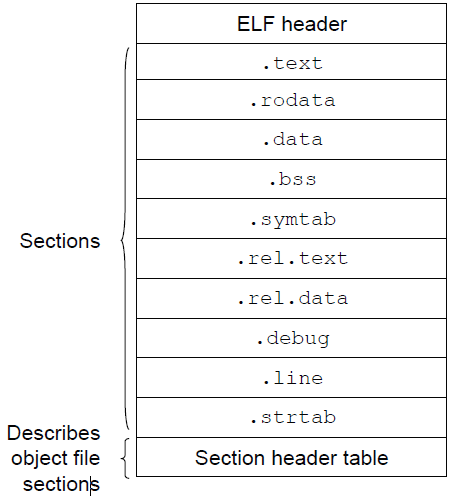
\includegraphics[scale=0.6]{Grafiken/relocatableObjectFile.png}
\caption{Das Format eines typischen ELF relocatable object files}
\end{figure}
Ein ELF\footnote{ELF - Executable and Linkable Format} relocatable object file beginnt mit einer 16-Byte Sequenz:
\begin{itemize}
\item Wort-Größe
\item Byte-Ordering
\item Weitere Infos für den Binder/Linker z.B. Maschinentyp
\end{itemize} 

Die einzelnen Segmente des files haben folgende Bedeutung:
\begin{itemize}
\item .text Maschinencode des compilierten/assemblierten Programms
\item .rodata Daten, welche nur gelesen werden müssen z.B. Formatierungsstrings oder Sprungtabellen für switch
\item .data Initialisierte globale Variablen
\item .bss\footnote{Block Storage Start, Better Save Space} Uninitialisierte globale Variablen
\item .symtab Symboltabelle mit Infos über Funktionen und globale Variablen
\item .rel.text Liste an Stellen, welche beim Linken modifiziert werden müssen, z.B. Kombination mit anderen files
\item .rel.data Relocations Informationen für globale Variablen
\item .debug Debugging Symboltabelle (Nur erzeugt, falls C-Compiler mit -g aufgerufen wurde)
\item .line Zuordnung der C-Anweisung zu Maschinencode (Nur falls -g gesetzt)
\item .strtab Zeichentabelle für Symboltabelle udn Debugging Symboltabelle
\end{itemize}

Diese Datei kann mit dem Befehl \textbf{readelf -h filename.o} geöffnet werden.\\
Mit \textbf{readelf -a filename.o} erhält man eine Übersicht über die wichtigsten Einträge.\\
Mit \textbf{objdump -S filename.o} erhält man den Maschinencode.\\

Analysewerkzeuge sind:
\begin{itemize}
\item IDA, ein kommerzieller Disassembler
\item Ghidra: Reverse-Engineering-Werkzeug der NSA
\end{itemize}

\subsection{Binder und Lader}

Der Binder (linker) hat die Aufgabe aus mehreren einzelnen verschiebbaren Objekt files ein ausführbares Objektprogramm zu erzeugen, indem die noch offenen externen Referenzen aufgelöst werden.\\
Das Objektprogramm kann dann durch einen Lader zur Ausführung gebracht werden.\\
Ein Lader (loader) ist ein Systemprogramm, welches Objektprogramme in den Speicher lädt und ggf. deren Ausführung anstößt.\\
Der Lader lädt ein Programmmodul (Lademodul) beginnend mit einer vom Betriebssystem vorgegebenen Startadresse in den Hauptspeicher.\\
Varianten sind:
\begin{itemize}
\item absolutes Laden
\item relatives Laden
\item dynamisches Laden zu Laufzeit
\end{itemize}

\subsection{Laufzeit}

Laufzeitmessungen von Programmen auf Assemblerebene können mit sogenanntem Programm Profiling durchgeführt werden.\\
Mit \textbf{gcc -pg -o functionname programmname.c} kann eine Objektdatei erzeugt werden, welche ein solches Profiling durchführt. Die Datei wird mit \textbf{./functionname} ausgeführt, dann lässt man sich mit \textbf{gprof functionname} die Profile Datei ausgeben.\\
Dies gibt Aufschluss über eventuelle Bottlenecks und zeigt Informationen wie z.B. die Zeit die das Programm in einzelnen Subroutinen verbracht hat. Aufbauend darauf kann dann z.B. Loop-Unrolling oder Thread Programmierung durchgeführt werden.

\section{Vorlesung 7}
\subsection{Microarchitekturen}
Die Befehlsausführung funktioniert grob in mehreren Schritten:
\begin{enumerate}
\item Befehlsholphase (instruction fetch): Das Steuerwerk liest die Befehle in den Speicher (Register)
\item Befehlsdekodierung (instruction decode): Dekodiert den Befehl
\item Befehlsausführung (instruction execute): Befehl wird ausgeführt, der nächste Befehl wird geholt
\end{enumerate}

Damit die Komponenten eines Rechnersystems kommunizieren können muss i.d.R. ein gemeinsamer Takt existieren.\\
Dieser wird als $f=\frac{1}{T}$, mit $T$ als Periodendauer bestimmt. Je höher der Takt, desto schneller werden Daten verarbeitet.\\
Der Leistungsumsatz ist $P\approx U^2 \cdot f \cdot C_L$.\\

Terminologie:
\begin{itemize}
\item ISA: instruction set architecture (Menge der verfügbaren Befehle)
\item RISC: reduced instruction set computer (kleine und schnell ausführbare ISA) z.B. ARM
\item CISC: complec instruction set computer (schwergewichtige ISA) z.B. Intel
\item SIMD: single instruction multiple data (vector processing) z.B. NEON
\item VLIW: very long instruction word (static multi-issue), superscalar processor
\item $\mu$arch microarchitecture (ISA Implementierung):
	\begin{itemize}
	\item Anzahl der Befehle pro Zyklus (IPC)
	\item Pipelining für Instruktionslevel Parallelismus (ILP)
	\item Sprungvorhersage
	\item out-of-order execution von Befehlen 
	\item multi-issue systems (startet mehrere Befehle pro Zyklus)   
	\end{itemize}
\end{itemize}

Wir unterscheiden verschiedene Architekturen:
\begin{itemize}
\item Eintakt-Implementierung/-Prozessor: Jeder Befehl wird in einem Takt ausgeführt
\item Mehrtakt-Implementierung: Jeder Befehl wird in Teilschritte zerlegt
\item Pipelined-Implementierung: Jeder Befehl wird in Teilschritte zerlegt und diese parallel ausgeführt
\end{itemize}

Die Ausführungszeit eines Programmes ergibt sich als:\\
Ausführungszeit = (\#Instruktionen) $\cdot$ (Takte pro Instruktion) $\cdot$ (Sekunden pro Takt)\\

Takte pro Instruktion $:=$ CPI\footnote{cycles per instruction}\\
Sekunden pro Takt $:=$ Taktperiode\\
$\frac{1}{CPI}$ = Instruktionen pro Takt = IPC\footnote{instructions per cycle}

\subsection{Eintaktprozessor}
\label{Architekturzustand}
Mit dem Architekturzustand bezeichnen wir die für den Programmierer zugänglichen Daten.
Dazu zählen:
\begin{itemize}
\item PC - Programm Counter
\item 16 Register
\item Speicher
\end{itemize}

Wir unterscheiden zwei Speichersysteme:
\begin{itemize}
\item Von-Neumann-Architektur
	\begin{itemize}
	\item gemeinsamer Speicher für Maschinenbefehle und Daten
	\end{itemize}
\item Harvard-Architektur
	\begin{itemize}
	\item Befehlsspeicher und Datenspeicher sind getrennt
	\end{itemize}
\end{itemize}

Dabei kann der Speicher bezogen auf den Takt asynchron gelesen werden, aber nur synchron geschrieben werden.\\

\subsubsection{Entwicklung des Datenpfades am Eintaktprozessor}

\begin{figure}[h!]
\centering
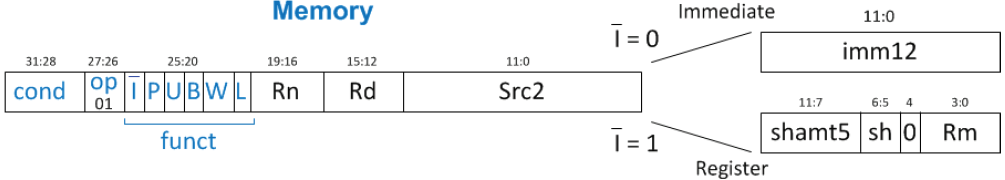
\includegraphics[scale=0.5]{Grafiken/ldr-Befehl.png}
\caption{Aufbau des ldr Befehls, n:m bezeichnet, dass der Bereich Bit m bis n umfasst}
\label{ldrBefehl}
\end{figure}

Wir beginnen mit der Entwicklung des Datenpfades für den LDR (ldr Rd, [Rn, imm12]) Befehl:\\
Im ersten \textcolor[rgb]{1, 0.7098, 0.4392}{hell-orange} markierten Schritt wird der Befehl im neuen Takt vom Instruction Memory geholt.\\
Im zweiten \textcolor[rgb]{0.1765,0.4627,0}{dunkel grün} markierten Schritt wird der Quell-Operand Rn vom Register file gelesen.\\
Im dritten \textcolor[rgb]{0,0.4314,0.6863}{cyan blau} markierten Schritt wird der Offset ausgewertet und zur weiteren Benutzung auf 32 Bit extended. Außerdem legen wir die Zieladresse an den passenden Port A3 an.\\
Im vierten \textcolor[rgb]{1,0,0}{rot} markierten Schritt wird der erweiterte Immendiate mit der Basisadresse RD1, welche vom Register file aus der an A1 anliegenden Registernummer ermittelt wird, addiert um die tatsächliche Adresse zu erhalten.\\
Im fünften \textcolor[rgb]{0.2,0.2,1}{magenta blau} markierten Schritt gibt der Data Memory Block die an der Adresse liegenden Daten an WD3 (Write data 3) weiter. Außerdem wird das RegWrite Steuersignal auf 1 gesetzt um die Daten aus WD3 an die Zieladresse A3 zu schreiben.\\
Im sechsten \textcolor[rgb]{0,0.4,0.4}{dunkel cyan} markierten Schritt wird die Adresse des nächsten Befehls (PC + 4 Byte) berechnet und angelegt.\\
Im siebten \textcolor[rgb]{1,0.851,0.4}{mittel gelb} markierten Schritt wird der Prozessor um die Möglichkeit erweitert die PC Adresse zu verwenden (Sowohl Quelle als auch Ziel). Da per Definition in der ARM Architektur das Lesen am Register R15 den PC + 8 zurückgibt, muss hierfür die nächste Befehlsadresse um 4 Byte inkrementiert werden und an der entsprechenden Stelle am Register file angelegt werden. Da PC aber auch geschrieben werden kann, muss noch der entsprechende Pfad vom Data Memory Block zur Auswahl an einen Multiplexer angelegt werden.\\

Um dieses Rechnersystem nun um den Befehl store (str) zu erweitern, welcher den Wert vom ersten Operanden Rd an die ermittelte Adresse aus dem zweiten Rn und dritten Operanden imm12 schreibt, muss einer Verbindung zwischen Rd und A2 hergestellt werden. Außerdem muss dann die Adresse von RD2 nun an den Write Data WD Port angelegt werden. Dies geschieht im \textcolor[rgb]{1,0.6,1}{hell magenta} markierten Schritt.
\begin{figure}[h!]
\centering
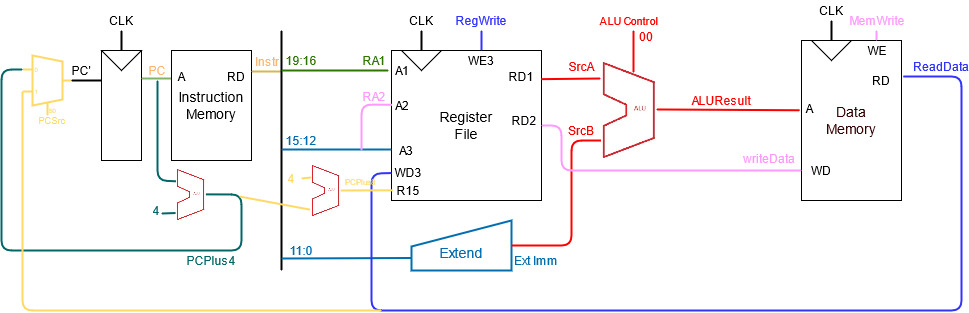
\includegraphics[scale=0.51]{Grafiken/strEintakt.jpg}
\caption{Eintaktprozessor für die Befehle ldr und str}
\end{figure}

Die Operation welche die ALU ausführt, wird mit folgenden über ALUControl gesteuerten Flags festgelegt:\\

\begin{tabular}{|l|l|}
\hline
$ALUControl_{1:0}$ & Function\\
\hline
00 & Add\\
01 & Subtract\\
10 & AND\\
11 & OR\\
\hline
\end{tabular}

%%if anything gets added above this needs to be removed
\newpage

\begin{figure}[h!]
\centering
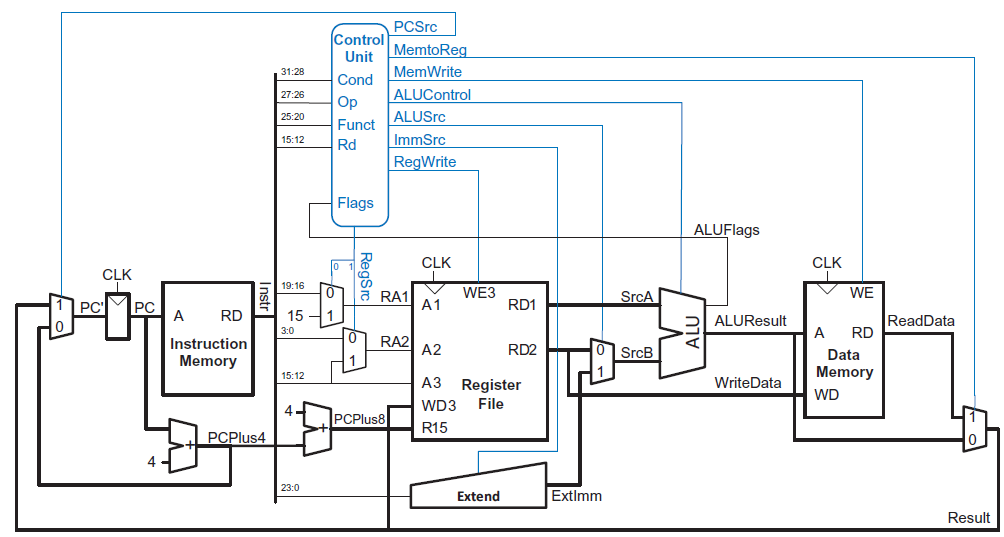
\includegraphics[scale=0.65]{Grafiken/Eintaktprozessor.png}
\caption{Der vollständige ARM Eintaktprozessor mit Kontrolleinheit}
\end{figure}


Die Flags der Kontrolleinheit haben folgende Bedeutungen:\\
{\footnotesize
\begin{tabular}{|l|l|l|}
\hline
Flag & Belegung & Bedeutung\\
\hline
PCSrc 	& 0 & PC soll auf den im Programm nachfolgenden Befehl zeigen\\
 		& 1 & PC soll auf eine berechnete Stelle im Programm zeigen\\
\hline
MemtoReg & 0 & Die Ergebnisdaten stammen aus einer Berechnung der ALU (z.B. ADD)\\
		& 1 & Die Ergebnisdaten stammen aus einem Register (z.B. LDR)\\
\hline
MemWrite & 0 & Gebe Daten über RD weiter an die Register File\\
		& 1 & Schreibe die Daten welche an der Adresse WD liegen in die Adresse A\\
\hline
ALUSrc & 0 & Verwende einen Wert aus einem Register für die Berechnung\\
	 & 1 &  Verwende den erweiterten Direktwert für die Berechnung\\
\hline
ImmSrc & 00 & Erweitere um 24 0-Bits bei arithmetischen/logischen Befehlen ($\{24'b0, Instr_{7:0}\}$)\\
	 & 01 & Erweitere um 20 0-Bits bei ldr/str Befehlen ($\{20'b0, Instr_{11:0}\}$)\\
	 & 10 & Erweitere um 6 Vorzeichenbits bei Branch ($\{6\{Instr_{23}, Instr_{23:0}\}\}$)\\
\hline
RegWrite & 0 & Es soll nicht ins Zielregister geschrieben werden\\
		& 1 & Das an WD3 anliegende Ergebnis soll in das Zielregister A3 geschrieben werden\\
\hline
RegSrc & 0 & Es existiert ein zweiter Operand, welcher vom Zielregister verschieden ist (z.B. ADD)\\
		& 1 & Es sollen Werte aus dem Zielregister ausgelesen werden (z.B. STR), bzw.\\
		& & es soll ein Sprung ausgeführt werden, d.h. nehme Wert aus R15 (PC), dann gleichzeitig\\
		& & ImmSrc = 10, MemtoReg = 0 und PCSrc = 1 um das Ergebnis zu übernehmen\\
\hline
\end{tabular}
}

Sprungbefehle:\\
Bei Sprungbefehlen wird der nächste PC durch eine Berechnung ermittelt. Dabei wird der zukünftige PC auch als BTA - Branch Target Address bezeichnet.\\
Diese wird als $BTA = (ExtImm) + (PC + 8)$ berechnet, wobei $ExtImm = Imm24 << 2$ (ImmSrc = 10) ist.

\subsubsection{Kontrolleinheit}
Die Kontrolleinheit setzt sich aus zwei Teilen zusammen, der Conditional Logic und dem Decoder.\\
Die Kontrolleinheit berechnet die Steuersignale entsprechend der cond, op und funct Felder im Befehl (\hyperref[ldrBefehl]{Bit $Instr_{31:20}$}), sowie der von der ALU generierten ALUFlags und dem Fakt ob der PC das Zielregister ist.\\
Die Conditional Logic speichert die ALUFlags und veranlasst nur eine Änderung des \hyperref[Architekturzustand]{Architekturzustands}, wenn die Instruktion nur bedingt ausgeführt werden soll.\\
Der Decoder generiert Steuersignale basierend auf der Instruktion.\\

\begin{figure}[h!]
\centering
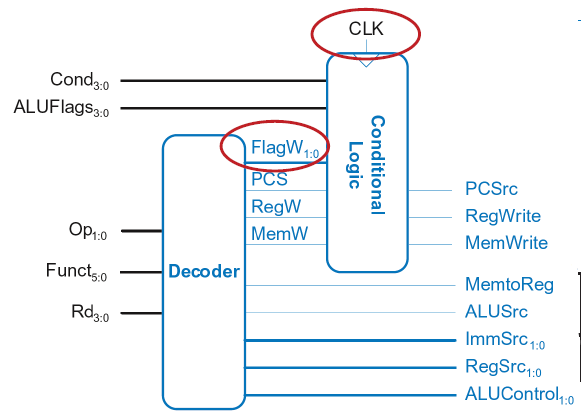
\includegraphics[scale=0.8]{Grafiken/Eintakt-Kontrolleinheit.png}
\caption{Die Kontrolleinheit des Eintaktprozessors}
\end{figure}

Die $FlagW_{1:0}$ Information gibt an, welche ALUFlags (NZCV) gespeichert werden sollen.\\
Die ADD, SUB Befehle updaten alle Flags, wohingegen AND, ORR nur NZ verändern können. Daraus ergibt sich folgende Interpretation:\\ $FlagW_1 = 1$ NZ ($ALUFlags_{3:2}$) wird gespeichert\\ $FlagW_0 = 1$ CV ($ALUFlags_{1:0}$) wird gespeichert

\begin{figure}[h!]
\centering
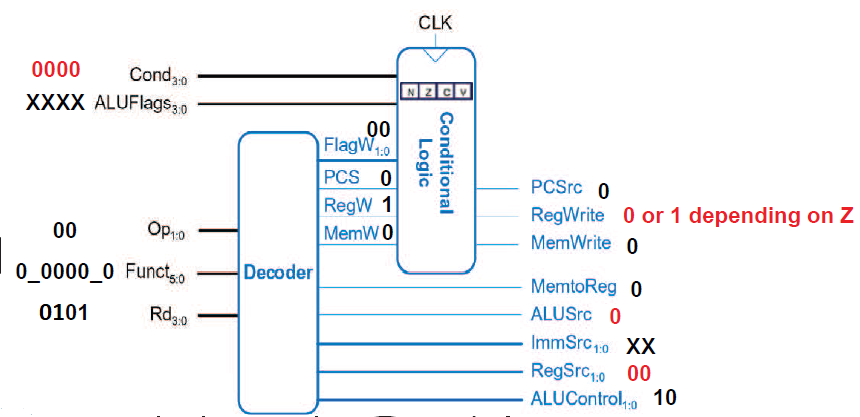
\includegraphics[scale=0.6]{Grafiken/Eintakt-Kontrolleinheit_Belegung-ANDEQ.png}
\caption{Beispielbelegung der Kontrollsignale für den Befehl: ANDEQ r5, r6, r7}
\end{figure}
Die Belegung von Cond, Op, Funct ergibt sich aus den \href{http://www.heenes.de/ro/material/arm/arm-instructionset.pdf}{Datenblättern}.

\section{Vorlesung 8}
\subsection{Mehrtaktprozessor}

Im folgenden Mehrtaktprozessor wird keine Harvard-Architektur, sondern eine Von-Neumann-Architektur\footnote{D.h. gemeinsamer Instruktions- und Datenspeicher} verwendet und ist auch heute weiter verbreitet. Trotzdessen könnte ein Mehrtaktprozessor auch eine Harvard-Architektur sein.\\
Ein Eintaktprozessor kann hingegen keine Von-Neumann-Architektur sein, da so im selben Takt auf zwei verschiedene Adressen zugegriffen werden müsste.

\begin{figure}[h!]
\centering
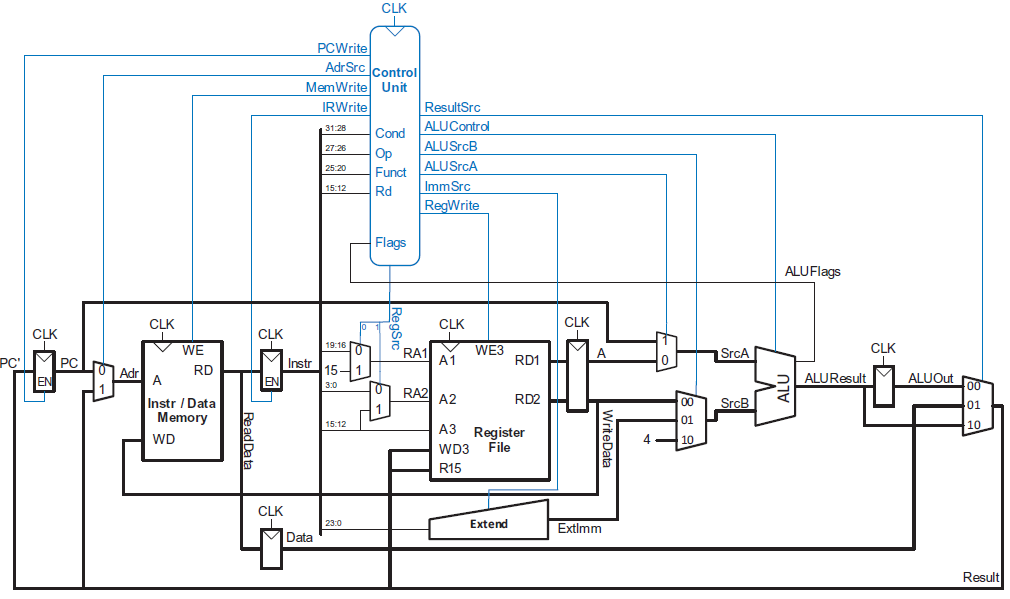
\includegraphics[scale=0.6]{Grafiken/Mehrtakt.png}
\caption{Ein Mehrtakt-Prozessor mit Kontrolleinheit}
\end{figure}

\begin{figure}[h!]
\centering
\includegraphics[scale=0.6]{Grafiken/Mehrtakt-Kontrolleinheit.png}
\caption{Aufgeschlüsselte Kontrolleinheit des Mehrtaktprozessors}
\label{fig:kontrolleinheit}
\end{figure}

Die Kontrolleinheit des Prozessors basiert auf einer FSM, welche die einzelnen Phasen der Befehlsausführung modelliert und die Steuersignale entsprechend der Phase vorgibt. Jede Phase wird durch einen eigenen Zustand beschrieben, sodass der Prozessor die entsprechenden Aktionen ausführt.\\
\begin{figure}
\centering
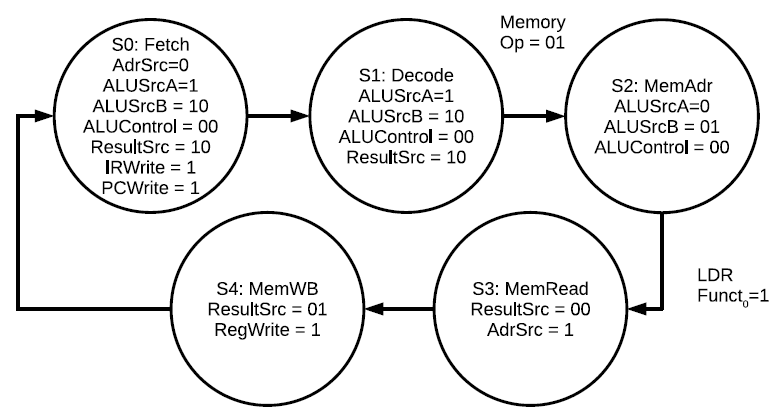
\includegraphics[scale=0.5]{Grafiken/Mehrtakt-Steuerwerk.png}
\caption{Das Steuerwerk für die Ausführung des Befehls ldr, welches das Verhalten der Kontrolleinheit in den einzelnen Ausführungsphasen beschreibt.}
\end{figure}

Ein Mehrtaktprozessor hat in der Regel eine höhere Taktfrequenz und einfache Instruktionen laufen schneller. Außerdem findet eine bessere Wiederverwendung von Hardware in verschiedenen Taktet statt, hat dafür jedoch eine aufwendigere Ablaufsteuerung.\\

Sie besitzen jedoch die selben Grundkomponenten.
\begin{itemize}
\item Datenpfad: verbindet funktionale Blöcke
\item Kontrollpfad: Steuersignale/Steuerwerk
\end{itemize}

%%if anything gets added further up this needs to be removed
\newpage

\section{Vorlesung 9}

\subsection{Pipeline-Prozessor}

Bei ARM wird die Befehlsausführung in fünf Schritte unterteilt:
\begin{enumerate}
\item Instruction Fetch
\item Instruction Decode, Read Register
\item Execute ALU
\item Memory Read/Write
\item Write Register
\end{enumerate}

Wir verwenden folgende Abkürzungen:
\begin{itemize}
\item IM - Instruction Memory (Befehlsspeicher)
\item RF - Register Field (Registerfeld)
\item DM - Data Memory (Datenspeicher)
\end{itemize}


\begin{figure}[h!]
\centering
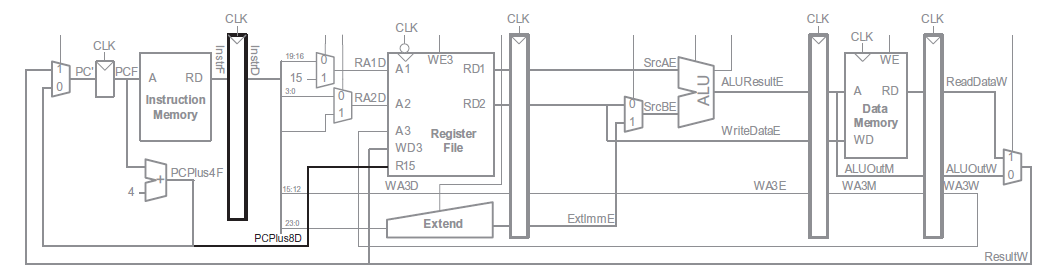
\includegraphics[scale=0.6]{Grafiken/PipelineProzessor-optimiert.png}
\caption{Ein optimierter Pipeline Prozessor, jede Pipelinestufe ist eine Stufe der Befehlsausführung.}
\end{figure}
Damit das richtige Writeback Register verwendet wird, wird dieses als WA3D durch die Stufen gereicht. Damit vom PC/R15 Register gelesen werden kann, könnten in die Fetch und Decode Pipelinestufen zwei Addierer den +8 Offset berechnen, oder wie hier den um +4 erhöhten PC des nächsten Befehls verwenden, und so einen Addierer sparen.

\begin{figure}[h!]
\centering
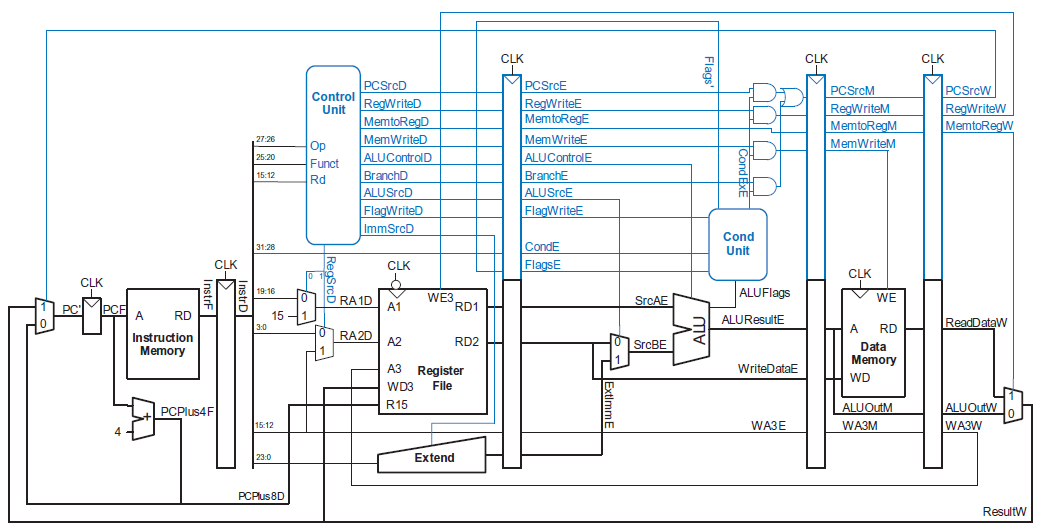
\includegraphics[scale=0.5]{Grafiken/PipelineProzessor-vollstaendig.png}
\caption{Der vollständige Pipeline Prozessor mit wie in \ref{fig:kontrolleinheit} dargestellt, aufgeteilter Kontrolleinheit.}
\end{figure}

\subsection{Hazards}
Hazards können beim Pipeline Prozessor auftreten, wenn eine Instruktion vom Ergebnis einer vorherigen abhängt, dieser aber noch kein Ergebnis geliefert hat.\\
Wir unterscheiden \textbf{Data Hazards} - Neuer Wert von Register noch nicht in Registerfeld eingetragen, und \textbf{Control Hazards} - Unklar welche Instruktion als nächstes ausgeführt werden muss.

\subsubsection{Data Hazard}
Ein Read-after-write Hazard (RAW) tritt auf, wenn eine vorherige Instruktion den neuen Registerwert noch nicht geschrieben hat, aber eine nachfolgende auf dieses Registerfeld zugreift.\\

Möglichkeiten um diesen Hazard zu umgehen sind:
\begin{itemize}
\item Wartezeiten einplanen, d.h. nops (no operations) zur Compile-Zeit einplanen und Ablaufplanung
\item Maschinencode zur Compile-Zeit umstellen (reordering)
\item Daten zur Laufzeit umleiten (bypassing)
\item Prozessor zur Laufzeit anhalten, bis Daten da sind (stalling)
\end{itemize}

Bei nops werden leere Instruktionen durch den Compiler in den Programmcode eingefügt, sodass benötigte Daten einen Takt weiter verarbeitet werden, und dann entsprechend aus dem Register gelesen werden können.\\

Beim Bypassing werden Ergebnisse aus anderen Pipelinestufen zu den benötigten Stellen weitergeleitet, um diese Ergebnisse dort zu verwenden, auch wenn diese noch nicht ins Register geschrieben wurden.\\

Beim stalling wird ein Schritt der Befehlsausführung, z.B. das Instruction Decode wiederholt um so einen zusätzlichen Takt für die Ausführung zu benötigen. Dadurch kann auf das Ergebnis eines Lade Befehls gewartet werden.

\begin{figure}[h!]
\centering
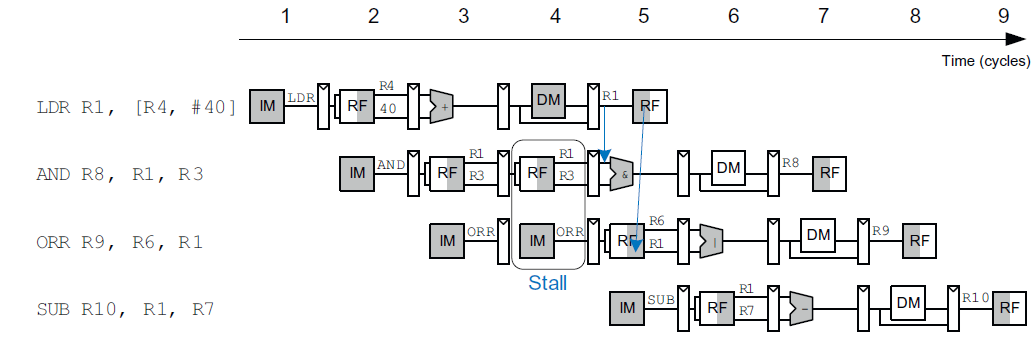
\includegraphics[scale=0.55]{Grafiken/Stalling.png}
\caption{Stalling zur Vermeidung eines Daten Hazards}
\end{figure}

\subsubsection{Control Hazard}

Bei einem Sprungbefehl werden die direkt nachfolgenden Instruktionen aufgrund der Natur des Prozessors geladen, aber ggf. nicht benötigt. Diese Instruktionen müssen nun aus dem Prozessor geflushed werden, also deren Ausführung unterbunden werden.\\
Bis das Ergebnis des Sprunges allerdings durch alle Pipelinestufen propagiert ist, dauert es mehrere Takte, obwohl das Ergebnis bereits früher vorliegt. Dies kann durch eine direkte Verbindung vom Addierer welche den PC mit dem Offset addiert, mit dem Register des nächsten PCs erreicht werden.\\

Damit dies möglich ist wird eine weitere Kontrolleinheit - die Hazard Unit benötigt.
\begin{figure}[h!]
\centering
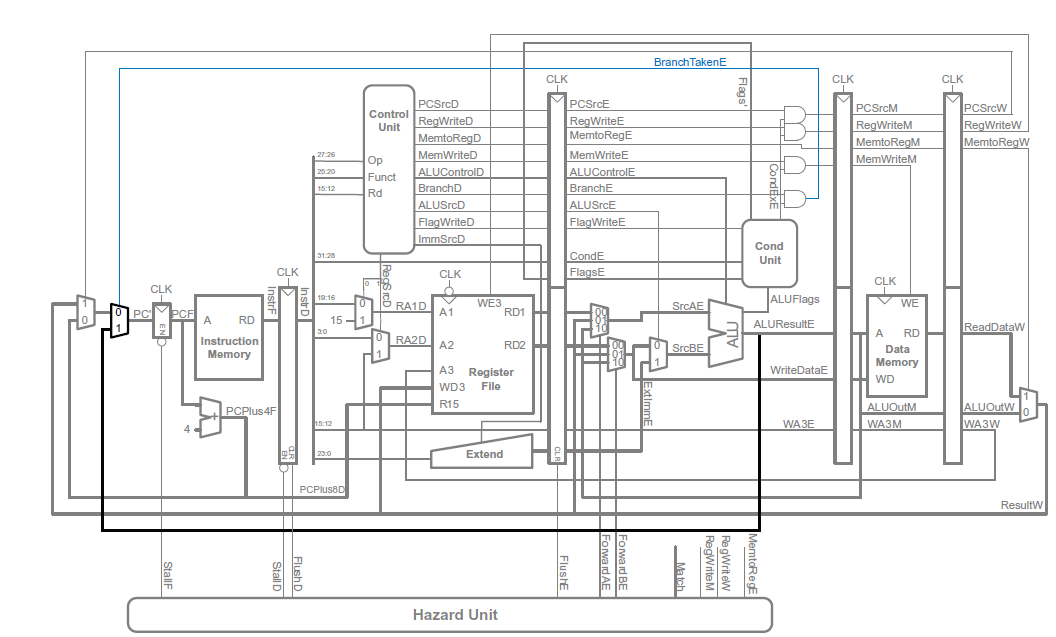
\includegraphics[scale=0.6]{Grafiken/HazardUnit.png}
\caption{Die Hazard Unit steuert die für die Hazard Bewältigung benötigten Signale}
\end{figure}

%%if anything gets added above this needs to be removed 
\newpage

\section{Vorlesung 10}
\subsection{Leistungsbewertung 1}
Leistungsfähigkeit sowohl von Hardware, als auch OS abhängig.\\
Einige Leistungskriterien für Rechnersysteme sind:
\begin{itemize}
\item Taktfrequenz $f=\frac{1}{T}$, T Periodendauer
\item Anzahl der Prozessoren
\item Größe und Art des Speichers
\item Antwortzeiten: Abhängig vom Aufgabentyp
\item Durchsatz: Relevanz im Rechenzentrum 
\item Ausführungszeit: Reine CPU Zeit ohne Ein-/Ausgabe
\end{itemize} 

Ausführungszeit bestimmt als:\\
\begin{itemize}
\item system CPU time: CPU-Zeit für Betriebssystemaufgaben
\item user CPU time: CPU-Zeit die zur Ausführung eines Programms benötigt wird
\end{itemize}

Leistungsumsatz:
$$P \equiv U^2 \cdot f \cdot C_L$$

Taktzyklen:\\
Für Eintakt \# Instruktionen = \# Takte\\
Für Mehrtakt ist $\frac{\text{Takte}}{\text{Instruktion}}$ = clock cycles per instruction (CPI)\\
$\frac{1}{\text{CPI}} = \frac{\text{Instruktionen}}{\text{Takt}} = \text{IPC}$ Instructions per cycle

Einfaches Maß ist MIPS - Million Instructions per second.

Bei der Klassifikation nach Flynn wird unterteilt in Instruction Streams und Data Streams.
\begin{itemize}
\item SI - Single Instruction
\item MI - Multiple Instruction (mehrere Befehle zu einem Zeitpunkt)
\item SD - Single Data
\item MD - Multiple Data
\end{itemize}

\begin{figure}[h!]
\centering
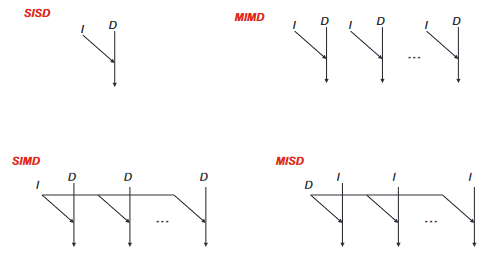
\includegraphics[scale=0.7]{Grafiken/Klassifikation-Flynn.png}
\caption{Veranschaulichung der Klassen von Flynn, MISD existiert nicht}
\end{figure}

\subsection{Betriebssysteme}

\begin{quote}
Die Programme eines digitalen Rechensystems, die zusammen mit den Eigenschaften der Rechenanlage die Grundlage der möglichen Betriebsarten des digitalen Rechensystems bilden und insbesondere die Abwicklung von Programmen steuern und überwachen. - Def. Betriebssystem nach DIN 44300
\end{quote}

Zu den Aufgaben des Betriebssystems gehören:
\begin{itemize}
\item Geräteüberwachung und -steuerung
\item Unterbrechungssteuerung
\item Ablaufsteuerung
\item Datenhaltung
\item Einhaltung von Qualitätsanforderungen
\end{itemize}

\begin{figure}[h!]
\centering
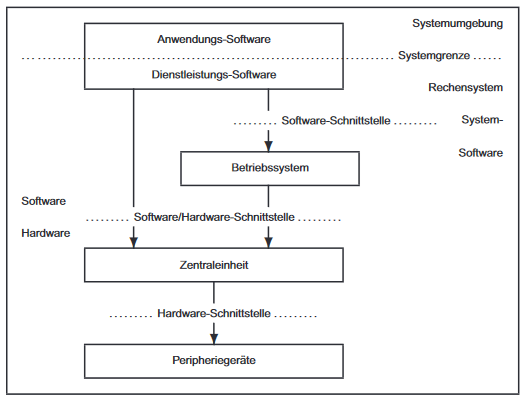
\includegraphics[scale=0.7]{Grafiken/VerfeinertesSchichtenmodell.png}
\caption{Darstellung des Schichtenmodells mit Schnittstellen zwischen Komponenten}
\end{figure}

Der Prozessor kann sich in verschiedenen Betriebszuständen befinden:\\
Maschinenzustand, der Prozessor kann aus/an geschaltet sein, oder laden\\
Privilegierungszustand:
\begin{itemize}
\item Anwenderzustand: nicht privilegiert, nur eingeschränkter Befehlsvorrat
\item Systemzustand: privilegiert, voller Befehlsvorrat
\end{itemize}
Ein Befehl heißt privilegiert, wenn er ausschließlich im Systemzustand ausführbar ist.

\newpage

\subsection{Ausnahmebehandlung}
Ohne Unterbrechungen ist die Arbeitsweise des Rechners:
\begin{enumerate}
\item Prozessor stößt Tätigkeit an
\item Gerät arbeitet selbständig, Prozessor muss warten
\item Prozessor arbeitet weiter
\end{enumerate}
Keine Parallelität und damit schlechte Ausnutzung des Prozessors.\\

Mit Unterbrechungen ist die Arbeitsweise:
\begin{enumerate}
\item Prozessor stößt Tätigkeit an
\item Gerät arbeitet selbständig, Prozessor arbeitet parallel weiter
\item Am Ende meldet sich das Gerät mit einer Unterbrechung beim Prozessor
\end{enumerate}

Ein solcher Interrupt ist ein Signal welches den Befehlszyklus des Prozessors abändert/unterbricht und diesen an einer bestimmten Stelle fortführt. Man unterscheidet grob:
\begin{itemize}
\item Programmbezogene Unterbrechungen (z.B. arith. Fehler, Adressfehler, falsche Befehle, ...)
\item Systembezogene Unterbrechungen (z.B. E/A-Unterbrechung, Prozessoranrufe, ...)
\item Maschinenfehler
\end{itemize}

Eine programmbezogene Unterbrechung trifft den Verursacher.\\
Systemaufrufe können auch als Interrupts zwischen nieder- und höherprivilegierten Zuständen wechseln, dadurch werden Dienste des Betriebssystems für den Benutzer verfügbar.

\section{Vorlesung 11}
\subsection{Zahlendarstellung}
Um auch reelle Zahlen darstellen zu können, muss ein Weg gefunden werden die Kommastelle zu repräsentieren.\\
Möglichkeiten hierzu sind:
\begin{itemize}
\item Festkommadarstellung
\item Gleitkommadarstellung
\end{itemize} 

\begin{figure}[h!]
\centering
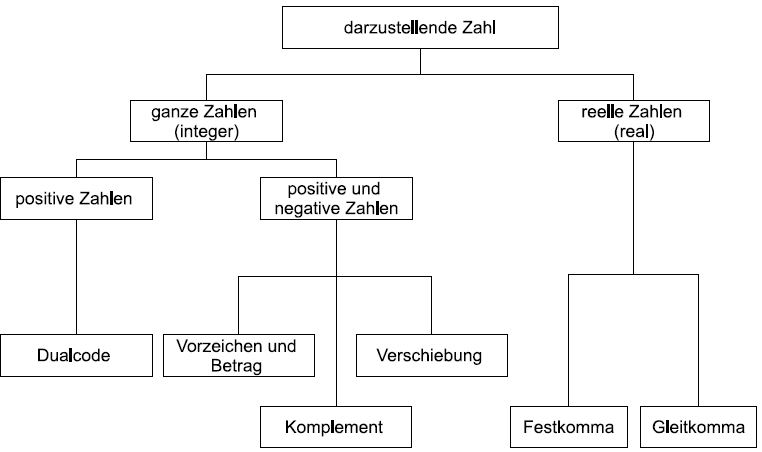
\includegraphics[scale=0.6]{Grafiken/Zahlendarstellung.png}
\caption{Zahlendarstellung in Rechnersystemen}
\end{figure}

Bei der Festkommadarstellung wird das Komma in der internen Zahlenabbildung weggelassen und man merkt sich wo es stehen müsste. Zum Programmbeginn wird die Kommastelle der entsprechenden Variablen definiert und bleibt dann während des Programms fest, deshalb \textbf{Fest}komma.\\

Bei der Gleitkommadarstellung auch halblogarithmische Darstellung ist die Kommastelle Bestandteil der Zahl und kann daher im Laufe der Zeit verändert werden. Diese Darstellung ist in ANSI/IEEE 754 spezifiziert und ist weltweit für den Datenaustausch und Rechenwerke standardisiert. Im Standard sind single, double und extended precision definiert.\\

Die Gleitkommadarstellung setzt sich aus dem Sign Bit (höchstwertige Position), dem biased Exponent und Fraction. 

\begin{figure}[h!]
\centering
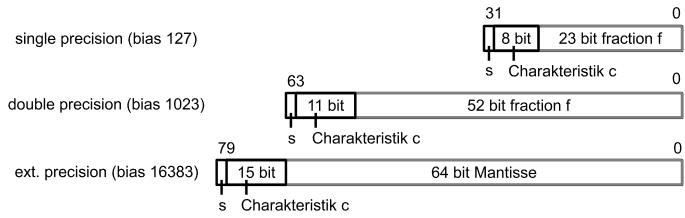
\includegraphics[scale=0.6]{Grafiken/IEEE754.png}
\caption{Precision im IEEE 754 Standard}
\end{figure}

Gleitkommazahlen in eingebetteten Systemen ohne Hardware-Unterstützung sollte vermieden werden.\\
Es existieren auch single precision Register (s0 - s31) und double precision register (d0 - d31) in Assembler, sowie passende Befehle für Addition (vadd.f64) und Loading, etc..\\
Der Befehl cpuinfo gibt Informationen über die CPU Architektur und Features an.\\

Gleitkommazahlen können entweder mit NEON oder VFP verarbeitet werden.

\subsection{Leistungsbewertung 2}

Leistungsmaße sind:
\begin{itemize}
\item Taktfrequenz
\item CPI Rate (Clock Cycles per Instruction)
\item MIPS Rate (Million Instructions per Second)
\item MFLOPS (Million Floating-point Operations per Second)
\end{itemize}

Zur Messungen können Benchmarks verwendet werden, wobei allerdings das Problem besteht dass häufig Compiler so optimiert werden, dass gängige Benchmarks schneller laufen. Arten von Benchmarks sind:
\begin{itemize}
\item Reale Programme
\item Kernels: kritische Auszüge aus realen Programmen
\item Toy Benchmarks: z.B. Quicksort
\item Synthetische Benchmarks: Spezielle Programme zur Leistungsevaluation
\end{itemize}

Benchmarks sind: SPEC, gzip und bzip.

BogoMips ist unwissenschaftlicher Benchmark, und ermittelt Wert beim Booten um Warteschleifen zu kalibrieren.

\subsection{NEON}

Dedizierte Funktionseinheit zur Beschleunigung der Berechnung von Ganz- und Gleitkommazahlen.
Beschleunigen Anwendungen der Signalverarbeitung, Videocodierung, etc.

NEON führt Packed SIMD aus, d.h. Register werden als Vektoren eines Datentyps betrachtet.\\
NEON hat 32 128 Bit Register welche auch paarweise kombiniert werden können.\\

Die Resultate von Operationen unterliegen der Saturations-Arithmetik.  Hierbei liegen alle Werte zwischen einem maximalen und minimalen Wert. Liegt ein Resultat einer Operation über dem Maximum wird es auf das Maximum gesetzt, liegt es unter dem Minimum auf das Minimum.\\

Neon kann auf vier Wege benutzt werden:
\begin{itemize}
\item NEON optimized libraries (OpenMax DL, Ne10)
\item Vectorizing compiler (gcc)
\item NEON intrinsics
\item NEON assembly
\end{itemize}
\end{document}